\section{Theorie}
\label{sec:Theorie}

Durch das Erwärmen von Metall können aus diesem Eletronen gelöst werden.
In einem Metall sind alle Atome in einer Gitterstruktur angeordnet.
Dies hat den Effekt, dass der Großteil der Atome ionisiert ist.
Die freigesetzten Elektronen hüllen dabei das Atomgitter ein und werden Leitungselektronen genannt.
Dabei wird angenommen, dass das Gitterpotential entgegen der Realität überall gleich ist.
So hat das Metallinnere ein posities Potential das sich um den Betrag $\phi$ von dem Potential des Außenraums unterscheidet.
Im Metallgitter wirken also keine Kräfte auf das Elektron.
Um aber das Metallgitter zu verlassen muss das Elektron gegen ein Potential $\Xi$ anlaufen, womit die Austrittsarbeit $e\Xi = W_\text{aus}$ definiert wird.
Diese Darstellung der Potentialunterschiede wird durch das Potentialtopf-Modell in Abbildung \ref{fig:potentialtopf} veranschaulicht.
\begin{figure}
    \centering
    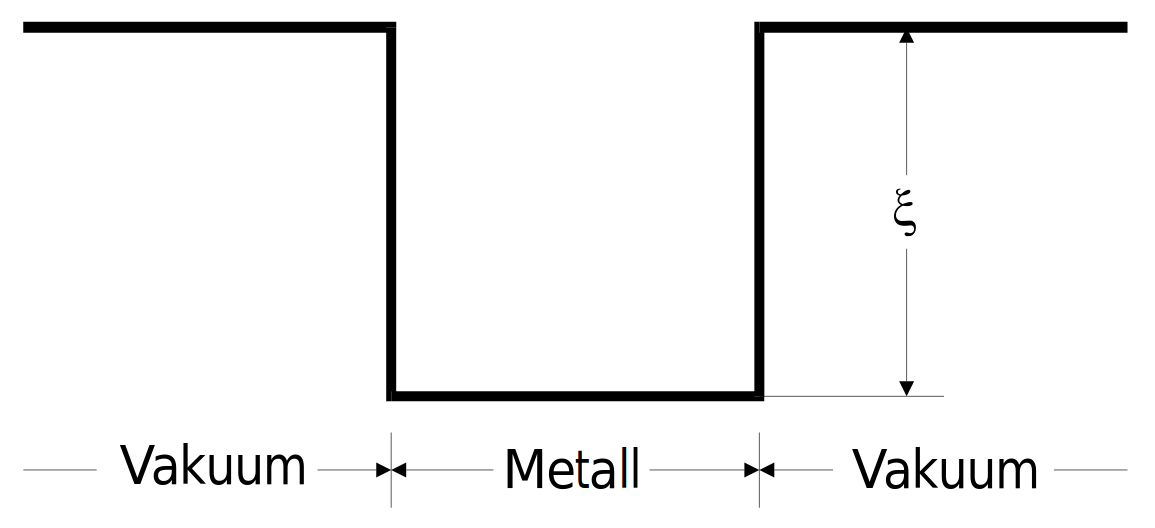
\includegraphics[width=0.4\textwidth]{content/data/potentialtopf.png}
    \caption{Potentialtopf-Modell eines Metall im Vakuum und Potential $\Xi$. Entnommen aus \cite[2]{anleitung}.}
    \label{fig:potentialtopf}
\end{figure}
\\\\
Dabei ist zu beachten, dass Elektronen einigen Gesetzmäßigkeiten folgen.
Zum Einem können Elektronen nur diskrete Energiezustände $E_\text{i}$ annehmen.
Zum anderen unterliegen sie dem Pauli-Verbot, welches besagt, dass immer nur zwei Eletronen einen Energiezustand $E_\text{i}$ besetzten können.
Dies steht im Widerspruch zu der klassischen Mechanik, in der jedes Elektronen im Mittel die Energie $\frac{3}{2} kT$ besitzt.
Dabei beschreibt $k$ die Boltzmannkonstante und $T$ die Temperatur.
Die beiden zuvor genannten Gesetztmäßigkeiten der Elektronen haben zur Folge, das Elektronen selbst bei $T=0$ eine endliche Energie besitzen.
Diese Grenzenergie $\nu$ hängt davon ab wie viele Elektronen sich in einem Volumenelemnt befinden.
Mit ihr kann die Fermi-Diracsche Verteilungsfunktion 
\begin{equation}
    f(E) = \frac{1}{\symup{e}^{\frac{E-\nu}{kT}} +1}
\label{eqn:fermi_dirac}
\end{equation}
aufgestellt werden.
Ihr Verlauf wird in Abbildung \ref{fig:fermi_dirac} gezeigt.
\begin{figure}
    \centering
    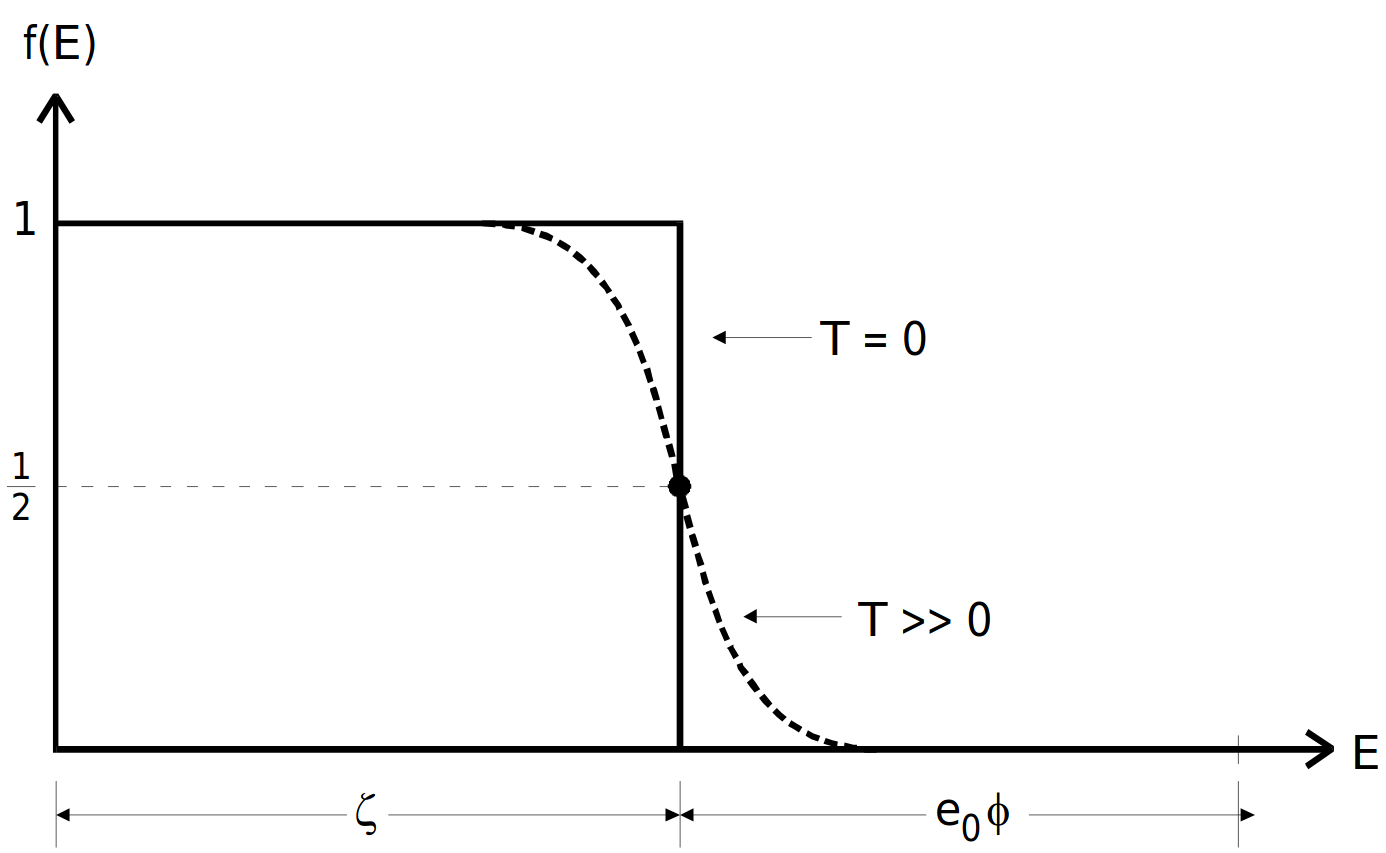
\includegraphics[width=0.4\textwidth]{content/data/fermi_dirac.png}
    \caption{Die Fermi-Diracsche Verteilungsfunktion am absoluten Nullpunkt und bei $ T > 0$. Entnommen aus \cite[3]{anleitung}.}
    \label{fig:fermi_dirac}
\end{figure}
Zu erkennen ist, dass ein Elektron mindestens die Energie $E = \nu + W_\text{aus}$ besitzen muss um das Metall zu verlassen.
Da selbst beim Schmelzpunkt von dem im Versuch zu betrachtenen Wolfram die Energiewerte noch groß gegenüber $kT$ sind kann eine weiter Näherung vorgenommen werden, aus der sich 
\begin{equation*}
    f(E) = \symup{e}^{\frac{\nu - E}{kT}}
\end{equation*}
ergibt.
\subsection{Stromdichte}
Um nun die Stromdichte $j_\text{s}(T)$ zu berechnen, also wie viele Elektronen pro Zieteinheit aus einer bestimmten Fläche austreten, wird das Metallgitter im dreidimensionalen Raum betrachtet.
Die Zahl der Elektronen $d\alpha$ die von Innen gegen die Metalloberfläche stoßen ist gegeben durch
\begin{equation}
    d\alpha = v_\text{z} N_\text{elek}\text{dx} \text{dy} \text{dz}.
    \label{eqn:dalpha}
\end{equation}
Dabei bilden $\text{dx} \text{dy} \text{dz}$ ein Volumenelement, $N_\text{elek}$ gibt die Anzahl der Elektronen pro Volumeneinheit ihres Phasenraumes an, $v_\text{z}$ gibt die Geschwindigkiet der Elektronen in Richtung der Oberflächennormale an.
Die Energie eines Elektron ist durch 
\begin{equation*}
    E = \frac{1}{2m_\text{elek}}\left ( p_\text{x} ^2 + p_\text{y} ^2 + p_\text{z} ^2 \right),
\end{equation*}
womit sich Gleichung \eqref{eqn:dalpha} zu 
\begin{equation*}
d\alpha = \symup{dE} N_\text{elek} \text{dx} \text{dy}
\end{equation*}
umformen lässt.
Jeder Qunatenzustand im sechsdimensionalen Phasenraum nimmt das Volumen $h^3$ ein, mit $h$ als Plankschen Wirkungsquantum.
So ergibt sich 
\begin{equation*}
d\alpha = \frac{2}{h^3}\symup{e} ^{\frac{\nu -E}{kT}} \text{dx} \text{dy} \symup{dE}
\end{equation*}
Aus dem Metall können allerdings nur Elektronen austreten, deren Impuls der Ungleichung
\begin{equation}
    \frac{p_\text{z}^2}{2m_\text{elek}} > \nu + e \phi
    \label{eqn:ungelich}
\end{equation}
Um nun die Stromdichte zu erhlaten werden alle Elektronen dessen Geschwindigkeit die Ungleichung \eqref{eqn:ungelich} erfüllen addiert und mit der Elementarladung multipliziert.
So ergibt sich für die Stromdichte, die sogeannte Richardson-Gleichung
\begin{equation}
    j_\text{s}(T) = 4\pi  \frac{e m_\text{elek}k^2}{h^3} T^2 \symup{e}^{\frac{-e\phi}{kT}}.
    \label{eqn:stromdichte}
\end{equation}
\subsection{Raumladungsdichte}
In Versuch wird mit einer Diode gearbeitet, diese hat die Eigenschaft, dass die Raumladungsdichte $\rho$ zur Anode hin abnimmt.
Dies liegt daran, dass die Elektronen zur Anode hin beschleunigt werden.
Aus der Kontinuitätsbedingung
\begin{equation*}
    -\rho = \frac{j}{v}
\end{equation*}
wird einsichtlich, dass bei höherer Geschwindigkeit $v$ und gleich bleibender Stromdichte $j$ also die Raumladungsdichte $\rho$ abnehmen muss.
Die Raumldungsdichte beeinflusst den Verlauf der Feldstärke zwischen Anode und Kathode.
Dadurch werden nicht alle Elektronen von dem Anodenfeld erfasst, dadurch ist der Diodenstrom kleiner als der zu erwartende Sättigungsstrom.
Um den Zusammenhang zwischen Anodenspannung und -strom zu ermitteln wird die Poisson-Gleichung
\begin{equation*}
    \Delta F = -\frac{\rho}{\epsilon_0}
\end{equation*}
herangezogen.
Hier gibt $F$ ein Potential und $\epsilon_0$ die Dielektrizitätskonstante des Vakuums an.
Diese wird vereinfacht indem angenommen wird, dass die Anode und Kathode unendliche weit ausgedehnte Platten sind, die sich im Abstand a gegenüberstehen.
Das Potential $F$ und die Raumladungsdichte $\rho$ hängen also nur noch von $x$ ab, so ergibt sich
\begin{equation*}
\frac{\symup{d^2F}}{\symup{dx}^2} = \frac{j}{\epsilon_0 v(x)}
\end{equation*}
wobei zusätzlich die Kontinuitätsbedingung genutzt wurde um $\rho(x)$ zu eliminieren.
Da der Energiesatz
\begin{equation*}
    eF = \frac{m}{2}v^2
\end{equation*}
kann die Gleichung zu 
\begin{equation*}
    \frac{\symup{dF}^2}{\symup{dx}^2} = \frac{j}{\epsilon_0 \sqrt{2eF/m}}
\end{equation*}
umgeschrieben werden.
Diese Gelichung kann nun nach einigen Umformungen integriert werden woraus sich schließlich das Lungmuir-Schottkysche Raumladungsgesetzt
\begin{equation*}
    j = \frac{4F^{3/2}}{9a^2}\epsilon_0 \sqrt{2e/m}
    \label{eqn:j}
\end{equation*}
ergibt.
Der Verlauf von Potential, Feldstärke und Raumladungsdichte in Abhängigkeit von x ist in Abbildung \ref{fig:ort_raum_feld} zu sehen.
\begin{figure}
    \centering
    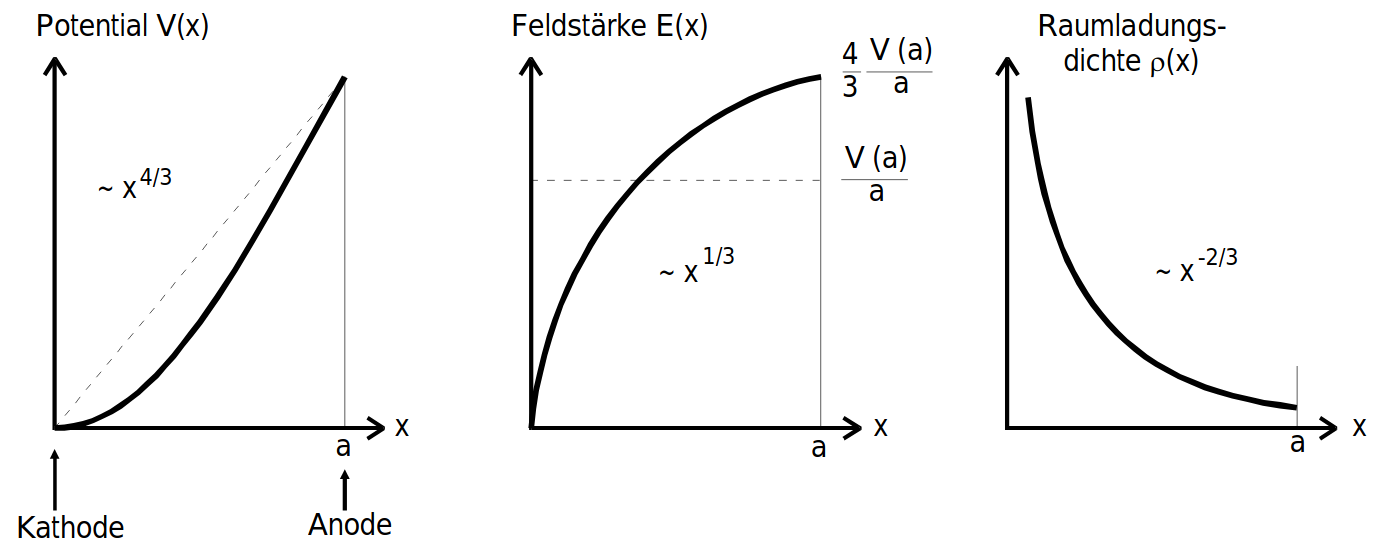
\includegraphics[width=0.5\textwidth]{content/data/Verlauf.png}
    \caption{Ortsabhängigkeit}
    \label{fig:ort_raum_feld}
\end{figure}

\subsection{Anlaufstrom}
Es ist zu beobachten, dass selbst wenn kein Potential anliegt ein Strom fließt.
Dies geht nicht aus der Gleichung \eqref{eqn:j} hervor, da der Grund für diesen Strom die kinetische Energie der Elektron im Metall ist.
Der Strom, welcher so zustande kommt wird Anlaufstrom genannt.
So können alle Elektronen die eine Energie
\begin{equation*}
    E > \ne + e\phi
\end{equation*}
aus dem Material austreten und bei genügend hohem $E$ sogar gegen ein kleines Gegenfeld anlaufen und die Anode erreichen.
Da zusätzlich meistens die Anode aus einem anderen Metall als die Kathode besteht, weist sie eine andere Austrittsarbeit $\phi_\text{A}$ auf.
Daraus folgt das nur Elektronen deren Energie größer als die Summe $e\phi_\text{A}+eF$ bei der Anode ankommen.
Dies wird in Grafik \ref{fig:potential} veranschaulicht.
\begin{figure}
    \centering
    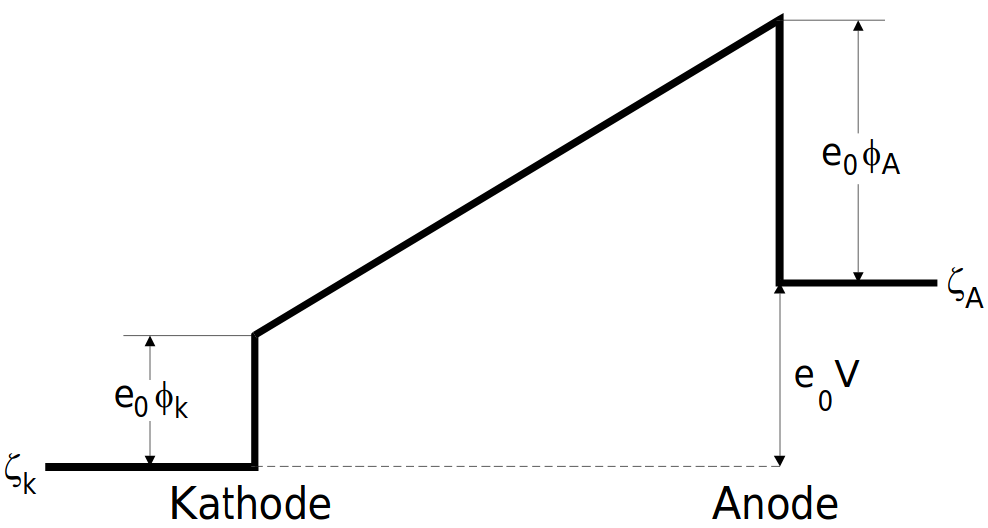
\includegraphics[width=0.5\textwidth]{content/data/potential.png}
    \caption{Potentialverhältnisse einer Anode und einer Kathode die aus Metallen mit verschiedenen Austrittsarbeiten bestehen. Entnommen aus \cite[8]{anleitung}.}
    \label{fig:potential}
\end{figure}
Aus diesem Zusammenhang kann nun eine Gelichung für die Anlaufstromstärke $j(V)$ aufgestellt werden
\begin{equation*}
    j(V) = j_0 \symup{e}^{-e\frac{\phi_\text{A}+V}{kT}}
\end{equation*}

\subsection{Kennlinie}
Aus den drei Bereichen Anlaufstrom, Raumladungsgebiet und Sättingstrom lässt scih nun die Kennlinie der Hochvakuumdiode zusammenstellen.
Ihr Verlauf ist in Abbildung \ref{fig:kennlinie} zu sehen.
\begin{figure}
    \centering
    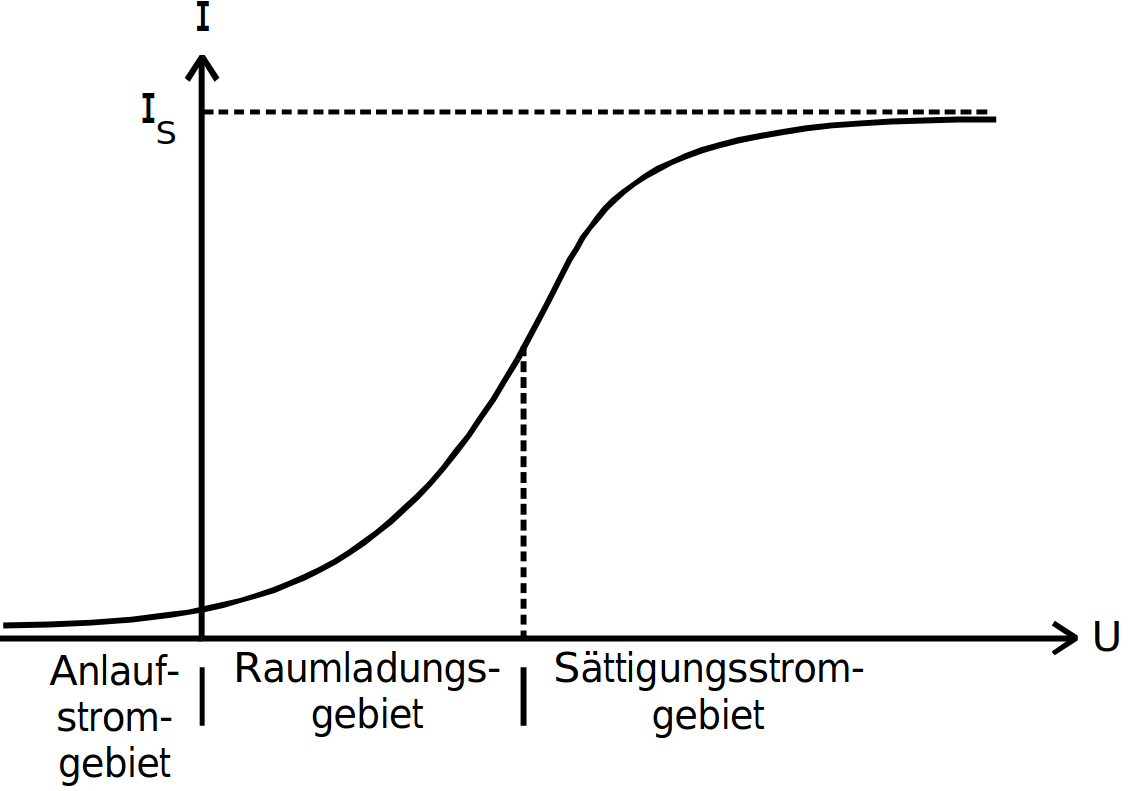
\includegraphics[width=0.4\textwidth]{content/data/kennlinie.png}
    \caption{Die Kennlinie einer Hochvakuumdiode, dabei wird der Diodenstrom in Abhängigkiet von der angelegten Spannung aufgetragen. Bild entnommen aus \cite[9]{anleitung}.}
    \label{fig:kennlinie}
\end{figure}
Dabei wird der Diodenstrom in Abhängigkeit von der angelegten Spannung aufgetragen.
Wie zu sehen ist kann die Kennlinie in die zuvor genannten Bereiche unterteilt werden.
Der Bereich des Anlaufstroms kennzeichnet sich durch den exponentiellen Zusammenhang zwischen $U$ und $I$ aus.
Der Darauf folgende Bereich das Raumladungsgebiet wird durch die Richardson-Gleichung \eqref{eqn:stromdichte} beschrieben.
Da aber die Richardson-Gleichung nicht für beliebig hohe Anodenspannungen gültig ist, strebt die Kennlinie bei einer gewissen Anodenspannung einem Sättigungswert entgegen.
So entsteht das Sättigungsstromgebiet.
